\documentclass{beamer}
\setbeamertemplate{navigation symbols}{}
\usepackage[latin1]{inputenc}
\usepackage{setspace,dsfont}
\usepackage{amsmath,amssymb,pdfpages}
\usepackage[longnamesfirst,nonamebreak]{natbib}
\usepackage[english]{babel}
\usepackage{eurosym,multirow,hyperref,cmll}
\usepackage{listings}
\usepackage{verbatim,booktabs}

\newcommand{\Lik}{\mathcal{L}}
\newcommand{\lau}{\lambda_u}
\newcommand{\wi}{\underline{w}}
\newcommand{\m}{\mathcal{M}}
\newcommand{\wa}{\overline{w}}
\newcommand{\lae}{\lambda_e}
\newcommand{\1}{\mathbb{1}}
\newcommand{\F}{\mathcal{F}}
\newcommand{\D}{\mathcal{D}}
\newcommand{\f}{\mathfrak{f}}
\newcommand{\E}{\mathbb{E}}
\newcommand{\V}{\mathbb{V}}
\newcommand{\N}{\mathbb{N}}
\newcommand{\Real}{\mathbb{R}}
\newcommand{\X}{\mathcal{X}}
\newcommand{\A}{\mathcal{A}}
\newcommand{\B}{\mathcal{B}}
\newcommand{\hy}{\hat{y}}

\hypersetup{
    colorlinks,%
    citecolor=blue,%
    filecolor=blue,%
    linkcolor=blue,%
    urlcolor=blue,
}
%\usetheme{Boadilla}
%\usetheme{Marburg}
%\usetheme{Hannover}
%\usetheme{Pittsburgh}
%\usetheme{umbc1}
%\usetheme{Montpellier}
%\usetheme{Singapore}
%\usetheme{}
%\usetheme{}
%\lstset {language=C++}

\DeclareMathOperator{\plim}{plim}
\DeclareMathAlphabet{\mathpzc}{OT1}{pzc}{m}{it}

\beamersetuncovermixins{\opaqueness<1>{25}}{\opaqueness<2->{15}}
\begin{document}
\begin{frame}
\title{ECON 613: Applied Econometrics}
\subtitle{Methods for Panel Data}
\titlepage
\end{frame}

\section{Linear Models}

\begin{frame}
\tableofcontents[currentsection] 
\end{frame}

\begin{frame}\frametitle{Introduction (1)}
\begin{itemize}
 \item Data on cross section that is observed over several unit of time.  
 \item In microeconometrics, panel are usually short. 
\end{itemize}
\end{frame}

\begin{frame}\frametitle{Introduction (2)}
\begin{itemize}
\item The error is correlated over time..
\item Examples
\item Open possibilities..
\end{itemize}
\end{frame}

\begin{frame}\frametitle{Introduction (3)}
Consider the following Model
\begin{equation}
 Y_{it} = \alpha_i + \gamma_{j(t)} + \beta X_{it} + \epsilon_{it}
\end{equation}
\begin{itemize}
 \item Estimation of fixed effects
 \item Correlation between the fixed effects
 \item Estimation issues
\end{itemize}
\end{frame}

\begin{frame}\frametitle{Introduction (4)}
Consider the following DGP:
\begin{itemize}
 \item 1,000 individuals over 10 periods. 
 \item $Y_{it} = \alpha_i + \beta X_{it} + \epsilon_{it}$
 \item Parametrization 
 \begin{itemize}
  \item $\beta = 1$
  \item $\alpha_i \sim uniform(0,1)$
  \item $\epsilon_i\sim \N(0,1)$
 \end{itemize}
\end{itemize}
\end{frame}

\begin{frame}\frametitle{Pooled Estimation}
\begin{table}
\begin{center}
\begin{tabular}{l c }
\hline
 & Model 1 \\
\hline
(Intercept) & $0.49^{***}$ \\
            & $(0.02)$     \\
c(xMat)     & $0.93^{***}$ \\
            & $(0.00)$     \\
\hline
R$^2$       & 0.87         \\
Adj. R$^2$  & 0.87         \\
Num. obs.   & 10000        \\
RMSE        & 1.05         \\
\hline
\multicolumn{2}{l}{\scriptsize{$^{***}p<0.001$, $^{**}p<0.01$, $^*p<0.05$}}
\end{tabular}
\caption{Statistical models}
\label{table:coefficients}
\end{center}
\end{table}
\end{frame}

\begin{frame}\frametitle{Fitted Values (1)}
\begin{figure}
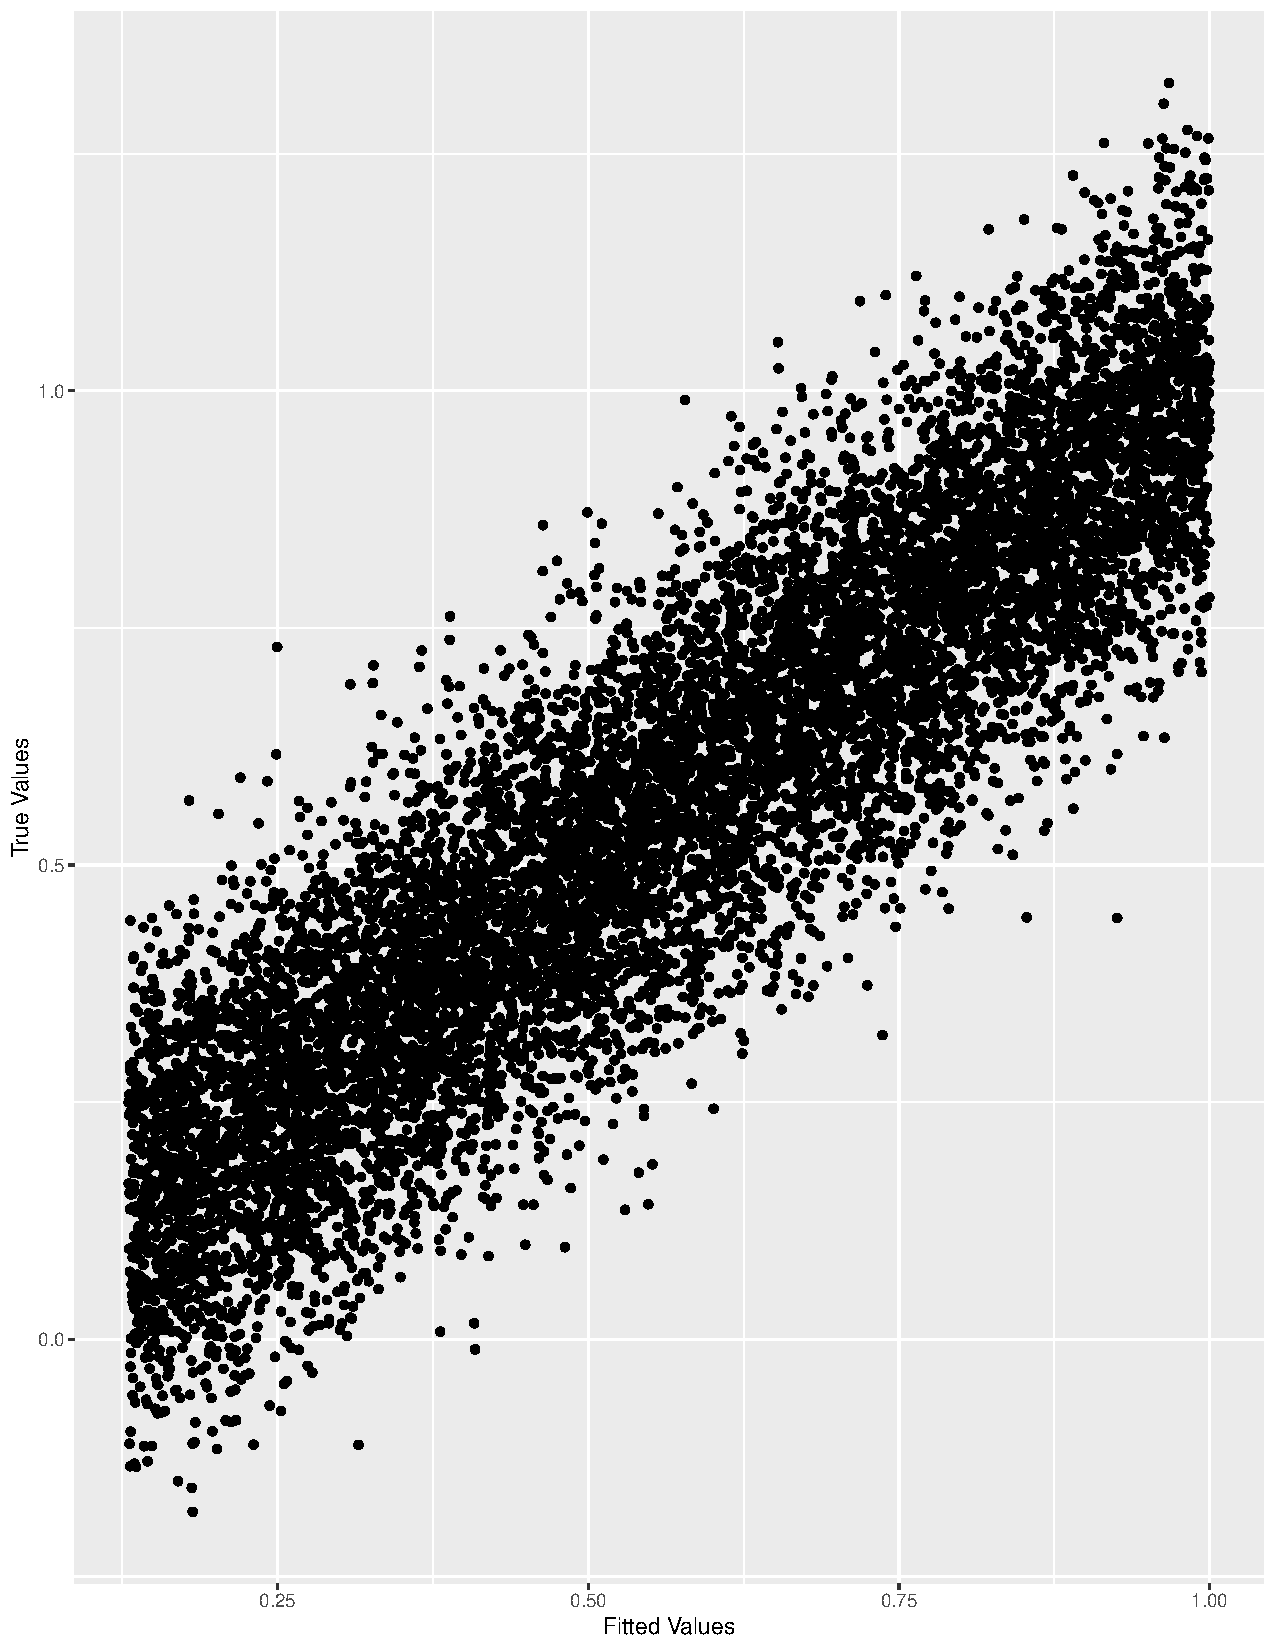
\includegraphics[width = 5cm]{plot/reg1}
\end{figure}
\end{frame}


\begin{frame}\frametitle{Introduction (5)}
Consider the following DGP:
\begin{itemize}
 \item 1,000 individuals over 10 periods. 
 \item $Y_{it} = \alpha_i + \beta X_{it} + \epsilon_{it}$
 \item Parametrization 
 \begin{itemize}
  \item $\beta = 1$
  \item $\alpha_i \sim uniform(-10,10)$
  \item $\epsilon_i \sim \N(0,1)$
 \end{itemize}
\end{itemize}
\end{frame}

\begin{frame}\frametitle{Pooled Estimation}
\begin{table}
\begin{center}
\begin{tabular}{l c }
\hline
 & Model 1 \\
\hline
(Intercept) & $-0.26^{*}$  \\
            & $(0.11)$     \\
c(xMat)     & $0.40^{***}$ \\
            & $(0.02)$     \\
\hline
R$^2$       & 0.04         \\
Adj. R$^2$  & 0.04         \\
Num. obs.   & 10000        \\
RMSE        & 5.73         \\
\hline
\multicolumn{2}{l}{\scriptsize{$^{***}p<0.001$, $^{**}p<0.01$, $^*p<0.05$}}
\end{tabular}
\caption{Statistical models}
\label{table:coefficients}
\end{center}
\end{table}
\end{frame}


\begin{frame}\frametitle{Fitted Values (2)}
\begin{figure}
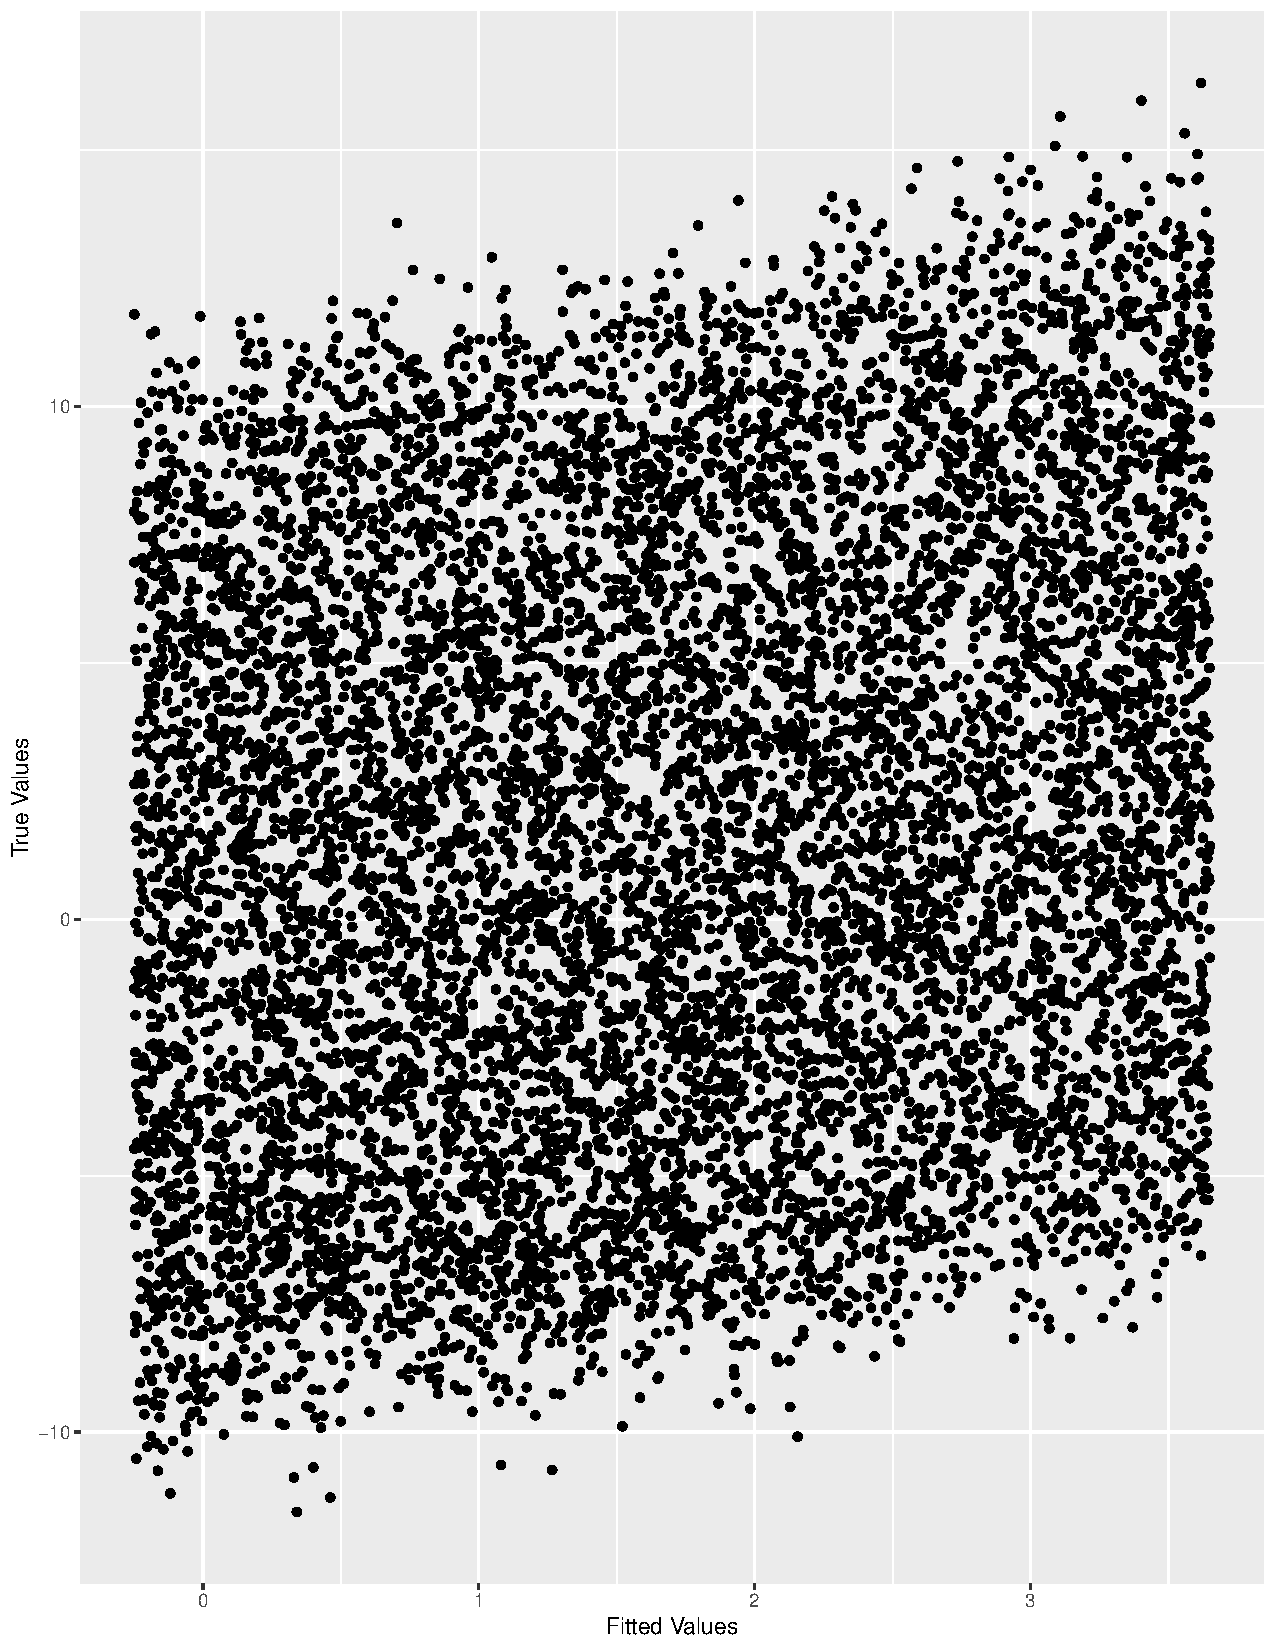
\includegraphics[width = 5cm]{plot/reg2}
\end{figure}
\end{frame}

\begin{frame}\frametitle{Effects}
\begin{itemize}
 \item Pooled Estimation is a good starting point.
 \item Individual VS Time Effect.
\end{itemize}
\end{frame}

\begin{frame}\frametitle{Individual Effects}
\begin{itemize}
 \item Fixed Effects
 \item Random Effects
 \item Examples: Return to Education
\end{itemize}
\end{frame}

\begin{frame}\frametitle{Time Effects}
\begin{itemize}
 \item Long Panel Case
 \item Example: Seasonality? 
\end{itemize}
\end{frame}

\begin{frame}\frametitle{Some Models (1)}
\begin{itemize}
 \item Pooled Estimator
 \begin{equation}
  Y_{it} = \alpha + \beta X_{it} + \epsilon_{it}
 \end{equation}
\item Problems
\end{itemize}
\end{frame}

\begin{frame}\frametitle{Some Models (2)}
\begin{itemize}
 \item Between Estimator
 \begin{equation}
  \hat{y}_i = \alpha_i + \beta \hat{x}_{i} + \hat{\epsilon}_{i}
 \end{equation}
\item Problems
\end{itemize}
\end{frame}

\begin{frame}\frametitle{Some Models (3)}
\begin{itemize}
 \item Within Estimator
 \begin{equation}
 y_{it} - \hat{y}_i =  \beta (x_{it} - \hat{x}_{i}) + 
 (\epsilon_{it} - \hat{\epsilon}_{i})
 \end{equation}
\item Problems
\end{itemize}
\end{frame}

\begin{frame}\frametitle{Some Models (4)}
\begin{itemize}
 \item First Difference Estimator
 \begin{equation}
 y_{it} - y_{i,t-1} =  \beta (x_{it} - x_{i,t-1}) + 
 (\epsilon_{it} - \epsilon_{i,t-1})
 \end{equation}
\item Problems
\end{itemize}

\end{frame}


\end{document}


